\documentclass[tikz,border=4pt]{standalone}
\usepackage{amsmath,amssymb,bm,setspace}
\usepackage{tikz,pgfplots}
\pgfplotsset{compat=1.18}
\usetikzlibrary{arrows.meta,calc,positioning,decorations.pathreplacing}
\begin{document}
% Case-A zero-lever response by achieved angular offset.
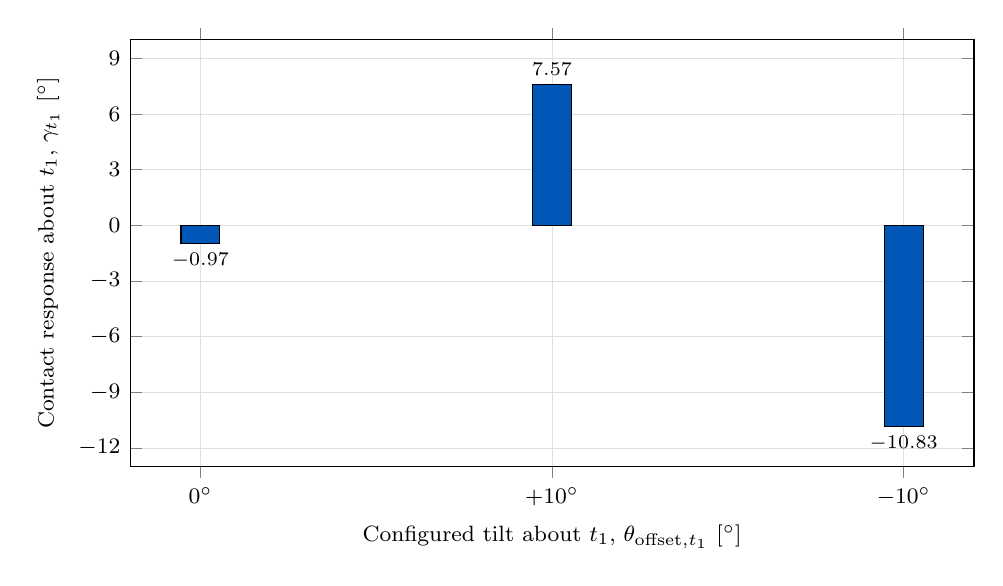
\begin{tikzpicture}
\definecolor{barblue}{HTML}{0057B8}
\begin{axis}[
    width=12.3cm, height=7.0cm,
    ybar,
    bar width=14pt,
    xtick=data,
    symbolic x coords={none, p10t1, m10t1},
    xticklabels={$0^\circ$,$+10^\circ$,$-10^\circ$},
    ymin=-13, ymax=10,
    ytick={-12,-9,-6,-3,0,3,6,9},
    grid=major,
    grid style={gray!25, very thin},
    tick label style={font=\footnotesize},
    label style={font=\footnotesize},
    % The three ticks carry two quantities: the zero-offset column is reported
    % by the magnitude \(\phi_0\), the other two by the \(t_1\) component.
    % Both are named, so no tick is labelled by a symbol that is not its own.
    xlabel={Configured tilt about $t_1$, $\theta_{\mathrm{offset},t_1}$ [$^\circ$]},
    ylabel={Contact response about \(t_1\), \(\gamma_{t_1}\) [\(^\circ\)]},
    nodes near coords,
    nodes near coords style={font=\scriptsize, /pgf/number format/fixed,
                             /pgf/number format/precision=2},
  ]
% The fill goes on the plot, not on every axis plot: the ybar cycle list sets
% its own fill at thirty per cent of the plot colour and is applied after an
% axis-level append style, which is why this figure rendered pale while the
% generated bar charts did not.
\addplot[draw=black, fill=barblue] coordinates {
  (none,-0.97) (p10t1,7.57) (m10t1,-10.83)};
\end{axis}
\end{tikzpicture}

\end{document}
